% ============================================================
% COMPUTATIONAL TOXICOLOGY – Special Issue: "Advancing FAIR and
% Integrative PBK Modelling for Next-Generation Risk Assessment"
% Submission deadline: 31 July 2026
% Article type to select in Editorial Manager: 'VSI: FAIR and PBK'
%
% FRAMING NOTES FOR AUTHORS:
% This paper (PBKFAIRModel + FAIRDatabase) is an excellent fit for Theme 1
% (FAIR Data and Model Standardization) and Theme 5 (Life-Stage and
% Population Variability) of the special issue. The PFAS early-life exposure
% model also directly addresses the special issue's explicit mention of PFAS as an emerging contaminant of interest.
%
% SUGGESTED FRAMING STRATEGY:
% - Lead with the FAIR-compliance angle: SBML encoding, open-source
%   web platform, role-based provenance tracking. This is the primary
%   contribution that distinguishes the paper.
% - Secondary angle: early-life (life-stage) pharmacokinetics for PFAS.
%   Explicitly position the breastfeeding/prenatal model as a demonstration of life-stage and population variability capabilities.
% - Tertiary angle: Integration with omics/microbiome data infrastructure
%   (FAIRDatabase), touching Theme 4 (New Approach Methodologies / multi-omics).
%
% MAIN MANUSCRIPT vs. SUPPLEMENTARY FILE SPLIT:
%
%   MAIN MANUSCRIPT should contain:
%     1. Abstract (≤250 words – currently too long, needs trimming)
%     2. Highlights (3–5 bullets, max 85 chars each)
%     3. Graphical Abstract (REQUIRED – currently missing, must be added)
%     4. Keywords (1–7, simple single-concept terms)
%     5. Introduction – motivation, FAIR gap, PFAS context, paper outline
%     6. Methodology:
%        - Brief model description (conceptual, not full ODEs)
%        - SBML encoding rationale (FAIRness argument)
%        - Integration architecture overview (FAIRDatabase)
%        - UI and API overview (summary table of endpoints)
%     7. Results & Discussion:
%        - Simulation outputs for 4 breastfeeding scenarios (fill in table!)
%        - FAIR compliance evaluation (checklist-style)
%        - Comparison with httk, IRRA frameworks
%        - Limitations
%     8. Conclusion
%     9. Declarations (CRediT, Funding, COI, AI use)
%     10. References (numbered, square brackets [1,2] style)
%
%   SUPPLEMENTARY FILE should contain:
%     S1. Full SBML module descriptions and ODE listing
%     S2. Complete table of all 64 state variables
%     S3. Complete API endpoint table (all 11 endpoints)
%     S4. Parameter values for PFOA and PFOS
%     S5. Full breastfeeding scenario parameterization table
%     S6. Installation and dependency instructions
%     S7. Python runner code listing (simulate_scipy.py excerpt)
%     S8. Role-based access control detailed table
%     S9. Subsubsubsection-level UI details (layout, CSV export, etc.)
%     S10. Zenodo Deposition Metadata 
% NOTE: The current manuscript has too many low-level technical details
% (package structures, Flask blueprint registrations, Jinja2 template names, etc.) in the main body. These belong in the supplementary file to keep the main text focused on scientific contribution and FAIRness demonstration.
% ============================================================

\documentclass[preprint,12pt]{elsarticle}

% ---- Elsevier elsarticle packages ----
\usepackage{graphicx}
\usepackage{multirow}
\usepackage{amsmath,amssymb,amsfonts}
\usepackage{mathrsfs}
\usepackage[title]{appendix}
\usepackage{xcolor}
\usepackage{textcomp}
\usepackage{pifont}
\renewcommand{\checkmark}{\ding{51}}
\usepackage{booktabs}
\usepackage{algorithm}
\usepackage{algorithmicx}
\usepackage{algpseudocode}
\usepackage{listings}
\usepackage{url}
\def\UrlFont{\rmfamily}
\usepackage{enumitem}
\usepackage{array}
\usepackage{lineno}
\usepackage{booktabs}
\usepackage{tabularx}
\usepackage{pdflscape}   % for \begin{landscape}
\usepackage{hyperref}    % for \href
\usepackage{setspace}
\usepackage{tikz}
\usepackage{pgfplots}
\pgfplotsset{compat=1.18}
\usetikzlibrary{shapes.geometric,arrows.meta,positioning,fit,backgrounds,shadows,calc}


% Elsevier natbib for numbered [1] style citations
% natbib loaded automatically by elsarticle; use \biboptions instead% natbib loaded automatically by elsarticle; \biboptions used below
\biboptions{numbers,sort&compress}

% ====================== JOURNAL METADATA ===================
% NOTE: Use elsarticle document class for Elsevier submission.
% Select journal: Computational Toxicology (ISSN 2468-1113)
% In Editorial Manager, select article type: 'VSI: FAIR and PBK'
% ============================================================

\journal{Computational Toxicology}

\begin{document}

\begin{frontmatter}

% ====================== TITLE ==============================
% NOTE: Title should be concise and informative. Avoid abbreviations
% unless firmly established (PFAS, SBML, FAIR are acceptable).
% Consider making the FAIR angle more prominent in the title for
% the special issue. Suggested alternative:
% "PBKFAIRModel: A FAIR-Compliant Web Platform for Early-Life
%  PFAS Exposure Assessment Using SBML-Encoded PBK Modelling"
% ============================================================
\title{\bfseries Integrating a PBK Module in FAIRDatabase Web Platform for Exposure Assessment: PFAS Case Study Across Pregnancy and Early Life}

% OLD TITLE: Integrating a FAIR-Compliant PBK Model into FAIRDatabase: Implementation and Web Interface for PFAS Exposure Assessment in Children

% ====================== AUTHORS ============================
% NOTE: Elsevier elsarticle uses \author and \address commands.
% Add ORCID IDs if available -- strongly encouraged by the journal.
% Mark corresponding author with \corref.
% ============================================================
\author[1,2]{Tu-Ky Ly}
\author[1,2,3,4]{Roland V. Bumbuc}
\author[2]{Senna Wiedeman}
\author[1,2]{Vivek M. Sheraton\corref{cor1}}
\ead{v.s.muniraj@uva.nl}
\cortext[cor1]{Corresponding author}

\address[1]{Computational Science Lab, Informatics Institute,
University of Amsterdam, Amsterdam, The Netherlands}
\address[2]{Informatics Institute, University of Amsterdam,
Amsterdam, The Netherlands}
\address[3]{Department of Plastic, Reconstructive and Hand Surgery,
Amsterdam Movement Sciences (AMS) Institute, Amsterdam UMC,
Location VUmc, Amsterdam, The Netherlands}
\address[4]{Department of Molecular Cell Biology and Immunology,
Amsterdam Infection and Immunity (AII) Institute, Amsterdam UMC,
Location VUmc, Amsterdam, The Netherlands}

\end{frontmatter}

% ====================== DATE ================================
% NOTE: Remove \date from the frontmatter; elsarticle handles dates.
% ============================================================

\begin{linenumbers}

% ====================== GRAPHICAL ABSTRACT =================
% ROLAND YOU ARE IN CHARGE! :)

% NOTE: A GRAPHICAL ABSTRACT IS REQUIRED by Computational Toxicology.
% It is currently MISSING from the manuscript.
% Create a single-panel figure (~500x400 px, min 300 DPI) showing:
%   - A schematic of the PBKFAIRModel workflow:
%     [SBML model] --> [Python runner] --> [FAIRDatabase] --> [Web UI]
%   - Small inset: example venous PFAS concentration curve for the
%     4 breastfeeding scenarios
% Submit as a separate image file (TIFF or EPS preferred, JPEG acceptable).
% ============================================================

% ====================== HIGHLIGHTS =========================
% NOTE: Required. Max 5 bullets, max 85 characters each (including spaces).
% Current bullets are within acceptable length but verify character count.
% Highlights must appear BEFORE the abstract in the submission system,
% uploaded as a separate file or in the cover letter system.
% ============================================================
\section*{Highlights} % --> TKL / Roland
\begin{itemize}
  \item ETL pipeline applied to PBK model FAIRification. 
  \item FAIR-compliant PBK model for PFAS encoded in SBML and deployed via Python.
  \item PFAS PBK parameter values standardized and stored in FAIRDatabase. 
  \item Web UI enables scenario configuration and interactive result visualisation.
  \item Role-based access control enabling collaborative, reproducible simulation workflows.
\end{itemize}

% ====================== ABSTRACT ===========================
% STRUCTURED ABSTRACT — fill in the [REPLACE: ...] blocks as results
% become available. Target: ≤250 words total. Current skeleton ~190 words.
%
% RESULTS BLOCK requires replication of four published studies:
%   [Study 1] Ratier et al. (2024)
%   [Study 2] Loccisano et al. (2013) 
%   [Study 3] Rovira et al. (2019) 
%   [Study 4] Ouidir et al. (2025) 
% Once these four replications are complete, replace [REPLACE: results]
% with quantitative outcomes (e.g., RMSE, % deviation from reference,
% peak C_ven values) and remove this comment block.
% ============================================================
\doublespacing

\begin{abstract} % --> TKL NEED TO CHANGE THIS!!!!!!

% --- BACKGROUND (≈50 words) ---
% Replace if framing changes; keep FAIR-first, PFAS-second structure.
Applying the FAIR (Findable, Accessible, Interoperable, Reusable)
principles to physiologically-based kinetic (PBK) models remains a
critical unmet need in computational toxicology. Existing PBK
implementations are siloed, lack persistent identifiers and open
interfaces, and cannot be directly linked to the biomonitoring data they
require for calibration and validation.

% --- OBJECTIVE (≈35 words) ---
% Replace only if scope changes.
PBKFAIRModel is presented: a FAIR-compliant lifetime PBK modelling
framework for per- and polyfluoroalkyl substance (PFAS) exposure
assessment, integrated into FAIRDatabase and demonstrated across
pregnancy and early life.

% --- METHODS (≈65 words) ---
% Replace the SBML/engine sentences only if implementation changes.
The model, originally developed by Beaudouin et al.\ and extended by
Ratier et al., was encoded in Systems Biology Markup Language (SBML)
Level~3 Version~2 and executed via an open-source Python simulation engine
deployed as a web platform within FAIRDatabase. Four breastfeeding
scenarios (none, 6~months, 1~year, 3~years) were configured for PFOA
and PFOS. Simulation runs are assigned persistent identifiers and stored
with full provenance metadata following FAIR Cookbook guidelines.

% --- RESULTS (≈40 words) ---
Simulated infant venous PFOA concentrations (Ratier et al.\ 2024 parameterisation)
declined from 10.9~ng/mL at birth to 1.1~ng/mL by age~7, consistent with
cord-blood inheritance and first-year elimination dynamics.
Rovira et al.\ (2019) maternal PFOA remained stable at 3.9~ng/mL throughout
gestation (GW12--38) with a fetal/maternal transfer ratio of 0.998.
Monte Carlo simulation of the Verner--Ouidir (2025) parameterisation
yielded mean maternal PFOS of 12.9~ng/mL at gestational month~1,
declining to 11.4~ng/mL at delivery, with a fetal mean of 5.0~ng/mL at term.

% --- CONCLUSIONS (≈40 words) ---
% Replace only if key claims change.
PBKFAIRModel provides an open-source, web-accessible PBK platform with
SBML-encoded model exchange, persistent storage, and provenance tracking,
contributing operationally to FAIR infrastructure for next-generation PFAS risk
assessment in vulnerable populations including pregnant women and infants.

\textbf{Keywords:} PBK modelling; FAIR principles; PFAS; early-life
exposure; SBML; open science; risk assessment
\end{abstract}

% ====================== KEYWORDS ===========================
% NOTE: Journal requires 1–7 keywords. Use single-concept terms.
% Avoid multi-word phrases with "and" or "of" where possible.
% Suggested keywords aligned with special issue keywords:
% PBK modelling; FAIR principles; PFAS; risk assessment; SBML;
% early-life exposure; web platform
% The current keyword list has 8 items and includes "pregnancy" and
% "microbiome" which are secondary to the main contribution -- consider
% replacing with "risk assessment" and "open science".
% ============================================================

% ====================== INTRODUCTION =======================

\section{Introduction}\label{sec1} % --> TKL

The assessment of chemical exposure during critical windows of development, particularly pregnancy and early childhood, requires elaborated computational approaches capable of linking external exposures to internal tissue concentrations across changing physiological states \cite{ratier2024,brochot2019,deepika2025}. 
Physiologically based kinetic (PBK) models have emerged as essential tools for this purpose, enabling quantification of internal dose, prediction of toxicokinetic behavior across life stages, and the support of regulatory risk assessment decisions \citep{beaudouin2010,deepika2022,beaudouin2024,brochot2019}. 
Per- and polyfluoroalkyl substances (PFAS) represent a particularly urgent case: these persistent synthetic chemicals, widely detected in human populations since the 1950s, have plasmatic half-lives of several years in humans, cross the placental barrier, accumulate in breast milk, and have been associated with diverse adverse health effects in children \citep{domingo2025,sunderland2019,lu2024,deSilva2021,panieri2022, habib2024,fenton2021,hasan2025,dehghani2025,kirk2018}. 
Reflecting this concern, the European Food Safety Authority (EFSA) derived its most recent tolerable weekly intake for four PFAS — PFOS, PFOA, PFNA, and PFHxS — directly from PBK model predictions accounting for infants as the critical sensitive population \citep{EFSA2020,deepika2025}. This further underscores that PBK models are embedded in regulatory decision-making for PFAS. The routes through which pregnant women and young children accumulate PFAS are multiple and temporally dynamic — transplacental transfer, breast milk, diet, and drinking water — and their relative contributions shift substantially as the child grows \citep{brochot2019,ratier2024}. 
Because blood sampling is invasive and ethically restricted in young children, human biomonitoring data for infants under two years of age remain particularly scarce, despite the first 1,000 days of life representing the most sensitive window of exposure to xenobiotics \citep{silveira2007,dePaula2026,jamnik2022,arbuckle2010}.
Furthermore, a single maternal plasma measurement at one time point can correspond to very different individual exposure histories, and internal doses in foetal target organs are rarely accessible to direct measurement \citep{brochot2019}. 
PBK modelling is therefore indispensable for characterising prenatal and early childhood internal PFAS dosimetry at the individual and population levels.

Over the past fifteen years, more than 28 PFAS PBK models was published for human populations \citep{deepika2025}, progressively extending from extrapolated-adult pharmacokinetics \citep{loccisano2011} to gestation and lactation in rat as a foundation to understand human PFAS toxicokinetic \citep{loccisano2013}, 
pregnancy \citep{verner2015}, 
individualized Bayesian reverse dosimetry \citep{brochot2019}, 
dietary multi-route exposure reconstruction using food frequency questionnaires \citep{rovira2019}, 
linking prenatal and childhood exposures in mother-child pairs \citep{ratier2024,ouidir2025}, 
and most recently mechanistic frameworks parameterized exclusively from \textit{in vitro} and \textit{in silico} data \citep{pachoulide2026}. 
Despite this scientific progression, the practical accessibility and reusability of these models remain severely limited. A recent systematic evaluation of 11 PFAS PBK models against the OECD guidance framework \citep{deepika2025} revealed that only approximately 55\% of assessed models provided replicable code, fewer than 45\% correctly reported units for both input and output parameters, and 65\% had never been used for any regulatory purpose. 
Models have been implemented in diverse software environments such as acslX, and GNU MCSim, with inconsistent parameters nomenclature, \textit{e.g.}, the plasmatic unbound fraction variously labeled "fu", "free", or "fup" across publications, and ultimately the absence of user-friendly platforms for reviewers to test models \citep{deepika2025}. Altogether, these inconsistencies among published models were identified as a primary barrier to regulatory uptake. 
A harmonised approach to PBK model reporting is urgently needed, with SBML \citep{hucka2003} explicitly recommended as the encoding standard to make models Findable, Accessible, Interoperable, and Reusable (FAIR) \citep{deepika2025}.

The FAIR principles \citep{wilkinson2016} have transformed data management across scientific disciplines, yet their application to computational models in toxicology remains fragile. Regulatory entities, such as the OECD, have published guidance for the validation and characterization of PBK models \citep{OECD2021}, and international initiatives such as the European Partnership for the Assessment of Risks from Chemicals (PARC, \citep{Ratier2023}) further underscore the urgency of FAIR-compliant model infrastructure. 
Concretely, "FAIRification" requires that models be findable through persistent identifiers, accessible via open interfaces, interoperable through community-standard formats, and reusable through clear provenance tracking and licensing, as outlined in the ELIXIR FAIR Cookbook \citep{rocca2023}. 
Beyond model encoding, standardized storage of input parameter sets is equally critical: PFAS PBK models require individual-level inputs, whose provenance and versioning must be traceable for results to be reproducible \citep{brochot2019,ratier2024}. Despite these frameworks, a persistent gap remains: no operational platform currently combines PBK model execution, standardized parameter storage, and interactive result visualisation within a single FAIR-compliant infrastructure for toxicokinetic modelling.

FAIRDatabase \citep{dorst2024,vanEldijk2026} was originally developed as an open-source, GDPR-compliant web platform for biomedical research data, implementing the FAIR principles through standardised storage, metadata management, and a privacy-preserving web interface~\citep{zhu2025fair}.  In this study, FAIRDatabase is extended to computational toxicokinetic modelling by integrating three published PFAS PBK models, 
spanning dietary multi-route exposure reconstruction in a Spanish pregnancy cohort \citep{rovira2019} based on 4 different models \citep{fabrera2014, fabrera2015,sharma2018a, sharma2018b}, pregnancy \citep{verner2015}, as applied in \citep{ouidir2025}, and a comprehensive mother-fetus-child framework applied to the HELIX cohort \citep{ratier2024}. 

PBK models were encoded in Systems Biology Markup Language (SBML) (Level 3 Version 2) and executed through a standardized open-source Python simulation engine \citep{hucka2003}. 
Published model parameters and simulation outputs are stored in the FAIRDatabase relational backend and exposed through an interactive web interface for scenario configuration, results visualisation, and data export. Reproducibility of the pipeline is demonstrated by comparing simulation outputs against published results for each study across all reported PFAS tissue concentrations. The platform is further assessed against each FAIRprinciple, discuss alignment with OECD model evaluation guidance, and outline perspectives for extending the approach to next-generation mechanistic models and integrated toxicokinetic-toxicodynamic applications.

This paper makes the following contributions:
(i)~SBML Level~3 Version~2 encoding of three published PFAS PBK model parameterisations (Ratier et al.\ 2024, Rovira et al.\ 2019, and Verner--Ouidir 2025), with unit-consistent parameter storage and structured provenance metadata in FAIRDatabase;
(ii)~a Python-native simulation engine capable of running all three parameterisations via a unified REST API, with each run assigned a persistent UUID and linked to the originating parameter set and SBML model version;
(iii)~integration into the FAIRDatabase open-source web platform, providing scenario configuration, interactive result visualisation, and CSV export within a FAIR-compliant, role-based access-controlled infrastructure;
(iv)~a reproducibility demonstration across four breastfeeding scenarios (none, 6~months, 1~year, and 3~years) and two PFAS compounds (PFOA, PFOS), with simulation outputs benchmarked against published reference values for each parameterisation; and
(v)~a structured assessment of PBKFAIRModel against the FAIR Guiding Principles and OECD PBK model evaluation guidance, identifying remaining gaps and a roadmap for next-generation model infrastructure.

\section{Materials and Methods}\label{sec2}

% ====================== METHODOLOGY ========================
% NOTE: This section needs significant restructuring for the journal.
% The current draft contains very deep technical detail (Flask blueprint
% registration, Jinja2 template names, Python package paths) that belongs
% in the Supplementary File (see S6, S7 below).
% Main text should present:
%   - Model conceptual description (compartments, ODEs, mass-balance)
on background layer%   - Integration architecture (conceptual, not code-level)
%   - UI overview (what a user can do, not how the HTML is structured)
% ============================================================
\subsection{FAIRDatabase Platform} % --> TKL
FAIRDatabase is an open-source, GDPR-compliant web platform~\citep{zhu2025fair} built on Supabase, originally developed as a FAIR-compliant data infrastructure for biomedical research \citep{dorst2024,vanEldijk2026}, incorporating federated learning capabilities to support privacy-preserving analyses across distributed datasets~\citep{de2026standardized,duah2025feddeepinsight}. It implements the FAIR principles \citep{rocca2023} through structured metadata management, controlled vocabulary, file format validation, and role-based access control (RBAC). Briefly, the backend uses Python (v3.10) with the Flask framework, and the platform is deployed locally to ensure GDPR compliance when handling sensitive participant data. Authentication is enforced via email-password login; two-factor authentication and Single Sign-On are available through the underlying Supabase platform configuration. Access is managed through a four-tier role hierarchy — Admin, Curator, Accessor, and Visualizer — restricting data entry and model parameterization to authorized contributors while keeping simulation outputs accessible to registered users. Full RBAC specifications are provided in the SI (Table SX).\\
In this study, FAIRDatabase is extended with a dedicated PBK modelling module, PBKFAIRModel, implemented as a Python package and registered as a Flask blueprint under the \texttt{/model} URL prefix. 
This extension follows the same design principles as prior FAIRDatabase modules \citep{vanEldijk2026}: server-side computation ensuring data remain within the secure platform environment, standardized storage of inputs and outputs in the relational backend, and an authenticated web interface for interactive use. The PBKFAIRModel package structure, REST API endpoints, and installation dependencies are detailed in the SI.




\subsection{PBK Model Architecture and SBML Encoding}\label{sec:model}

The lifetime PFAS PBK model, originally developed by Beaudouin et al.\ and extended by Ratier et al.\ (2024), describes whole-body PFAS kinetics using a system of first-order ordinary differential equations (ODEs) governing mass balance across seven physiological compartments: venous blood, arterial blood, liver, kidney, richly perfused tissues, slowly perfused tissues, and, during gestation and lactation, a foetal-placental unit and a mammary gland compartment. For each compartment $i$, the governing mass-balance equation takes the form:

\begin{equation}\label{eq:massbalance}
\frac{\mathrm{d}A_i}{\mathrm{d}t} = Q_i \left( C_{\mathrm{art}} - \frac{C_i}{P_i} \right) + S_i - E_i
\end{equation}

where $A_i$ denotes the amount of PFAS in compartment $i$ ($\mu$g), $Q_i$ the compartment-specific blood flow rate (L~h$^{-1}$), $C_{\mathrm{art}}$ the arterial blood concentration ($\mu$g~L$^{-1}$), $C_i$ the compartment concentration ($\mu$g~L$^{-1}$), $P_i$ the tissue-to-blood partition coefficient (dimensionless), $S_i$ a compartment-specific source term (for example, dietary absorption or placental transfer), and $E_i$ the elimination term (renal clearance or hepatic biotransformation). Renal clearance is governed by a first-order rate constant derived from published urinary excretion data. For PFOA and PFOS in humans, hepatic biotransformation is considered negligible and elimination follows a linear clearance term \citep{loccisano2011,ratier2024}.



Life-stage transitions, specifically the onset of pregnancy, gestational growth, parturition, and the initiation and cessation of breastfeeding, are implemented as time-dependent parameter functions within the ODE system. Physiological parameters including blood flow rates, organ volumes, and body weight follow trimester-specific trajectories based on established reference data for human gestation \citep{beaudouin2010,ratier2024}.

The model was encoded in Systems Biology Markup Language (SBML) Level~3 Version~2 using the libSBML Python application programming interface. SBML was selected as the exchange format because it provides a machine-readable, schema-validated representation of the model structure, parameter values, initial conditions, and unit definitions within a single, self-contained file. This encoding satisfies the Interoperability and Reusability criteria of the FAIR principles, enabling the model to be imported directly into SBML-compliant simulation environments, such as COPASI, Tellurium, or RoadRunner, without manual transcription. Unit consistency was verified against OECD guidance for PBK model reporting, with all rate constants expressed in h$^{-1}$, volumes in litres, concentrations in $\mu$g~L$^{-1}$, and flows in L~h$^{-1}$ \citep{OECD2021}. The SBML file includes structured \texttt{<notes>} elements providing chemical identity metadata (CAS number, InChI key, molecular weight) and a \texttt{<listOfModelHistory>} block recording authorship and versioning provenance \citep{hucka2003}.

Parameter values for PFOA and PFOS were drawn from the published literature and stored in the FAIRDatabase \texttt{pbk\_parameter\_sets} table with full schema documentation (Supplementary Table~S4). Each entry carries a chemical identifier, source reference, numerical value, and SI unit string, ensuring that stored parameter sets are independently interpretable without reference to the source code.

\subsection{Simulation Protocol}\label{sec:simprotocol}

Simulation execution is managed by a Python-native runner that loads the SBML model file, reads the selected parameter set from the FAIRDatabase backend, applies life-stage parameter overrides for the requested scenario, and integrates the ODE system using the LSODA solver as implemented in \texttt{scipy.integrate.solve\_ivp} with absolute and relative tolerances of $10^{-8}$ and $10^{-6}$, respectively. Integration proceeds over the specified simulation period with a fixed output interval of one day. Time-concentration profiles for all compartments are written to the \texttt{pbk\_runs} table in the relational backend, referenced by a unique simulation run identifier and linked to the originating parameter set identifier and SBML model version. The full set of solver configuration options is documented in Supplementary Section~S6.
% NOTE: Keep this section brief in the main text. Move subsubsection-
% level detail (layout, artifact upload file formats, CSV export
% mechanics, Chart.js configuration) to Supplementary Section S9.
\subsection{User Interface}\label{sec:ui}

The PBKFAIRModel user interface provides an accessible, interactive
experience for configuring and visualising PBK simulations without
requiring command-line access or programming expertise. Users configure
simulations through four inputs: breastfeeding scenario, chemical
half-life (years), dietary intake rate (ng/kg/min), and birth year.
Results are displayed as an interactive time-concentration profile
(Chart.js) with four summary statistics (peak concentration, age at
peak, final concentration, final age) and a full CSV export. Artifact
storage supports images, videos, and mesh files with role-gated access.

% ====================== RESULTS AND DISCUSSION =============
\section{Results and Discussion}\label{sec3}

\subsection{Simulation Results} % --> TKL
% TKL : describes the transcription of each of the 4 model in sbml + plot comparison of all outputs from the orignal 

To demonstrate the reproducibility of the PBKFAIRModel pipeline, simulation outputs were compared against published reference values for each of the four parameterisations integrated into FAIRDatabase. For each parameterisation, the SBML-encoded model was executed with the corresponding published parameter set stored in the \texttt{pbk\_parameter\_sets} table, using the four breastfeeding scenarios (no breastfeeding, 6~months, 1~year, and 3~years) specified in the original studies.

For the PFOA parameterisation derived from Ratier et al.\ (2024), the SBML-encoded runner was executed from birth to age~7 years (birth year~2007, $t_{1/2}=3.5$~years, dietary intake $R_{\mathrm{inj}}=0.452$~ng/kg/min). The simulated infant venous plasma PFOA concentration started at 10.9~ng/mL at birth (cord-blood transfer) and declined to 4.2~ng/mL at age~1, 2.8~ng/mL at age~2, and 1.1~ng/mL at age~7 years. This declining post-natal trajectory is consistent with the progressive elimination of cord-blood-inherited PFAS burden reported by Ratier et al.\ and the biomonitoring data of the HELIX cohort.

For the Rovira et al.\ (2019) maternal plasma PFOA parameterisation (initial $C_{V,\mathrm{init}}=4.0$~ng/mL, body weight 60~kg), the runner returned a stable maternal arterial plasma concentration of 3.9~ng/mL throughout gestation (GW12 and GW38), with a fetal/maternal transfer ratio of 0.998 at delivery. This near-unity transfer ratio is consistent with the high transplacental passage of PFOA reported in human studies and reproduced by the original Rovira model.

For the Verner--Ouidir (2025) parameterisation (PFOS, 50 Monte Carlo iterations, $t_{1/2}=5.4$~years), the population-level simulation yielded a mean maternal PFOS trajectory declining from 12.9~ng/mL at gestational month~1 to 11.4~ng/mL at term, with the 5th--95th percentile band spanning 4.8--20.5~ng/mL at month~1 and 4.4--19.4~ng/mL at term. Mean fetal arterial PFOS at term was 5.0~ng/mL, corresponding to a fetal/maternal ratio of 0.44, consistent with the values reported by Ouidir et al.\ and the reference ranges of Verner et al.

Figure~\ref{fig:simresults} presents concentration-time profiles for the three implemented studies. Figure~\ref{fig:bfscenarios} shows the infant venous PFAS trajectory from birth to age~7 under the four breastfeeding scenario configurations; numerical summary statistics for each run are presented in Table~\ref{tab:sim_summary}. The SBML encoding and database-mediated parameter retrieval were confirmed to introduce no computational artefacts relative to the original model implementations: all runs completed within the expected numerical precision of the LSODA solver ($r_\mathrm{tol}=10^{-6}$, $a_\mathrm{tol}=10^{-9}$).

\begin{table}[h]
\centering
\caption{Summary statistics of PBKFAIRModel simulation runs across three published parameterisations. All concentrations in ng/mL; fetal/maternal ratio is dimensionless. Ratier results are for the no-breastfeeding scenario; BF scenario differentiation in infant C\textsubscript{ven} is subject to ongoing validation (see Section~\ref{sec3}.4).}
\label{tab:sim_summary}
\small
\begin{tabular}{p{2.8cm} p{1.8cm} p{1.8cm} p{2.0cm} p{2.2cm}}
\toprule
\textbf{Parameterisation} & \textbf{Compound} & \textbf{Peak conc.\ (ng/mL)} & \textbf{Age/stage at peak} & \textbf{Final conc.\ (ng/mL)} \\
\midrule
Ratier et al.\ (2024) & PFOA & 12.2 & birth (age 0.03 yr) & 1.1 (age 6.8 yr) \\[3pt]
Rovira et al.\ (2019) & PFOA & 3.9 (maternal) & GW12 & 3.9 (GW38); cord blood 3.9 \\[3pt]
Verner--Ouidir (2025) & PFOS & 13.2 (mat.\ mean) & month 2 & 11.4 (month 9); fetal 5.0 \\
\bottomrule
\end{tabular}
\end{table}

% ============================================================
% FIGURE 2: 4-panel reproducibility comparison
% Stand-in figure: replace with actual simulation output data
% ============================================================
\begin{figure*}[htbp]
\centering
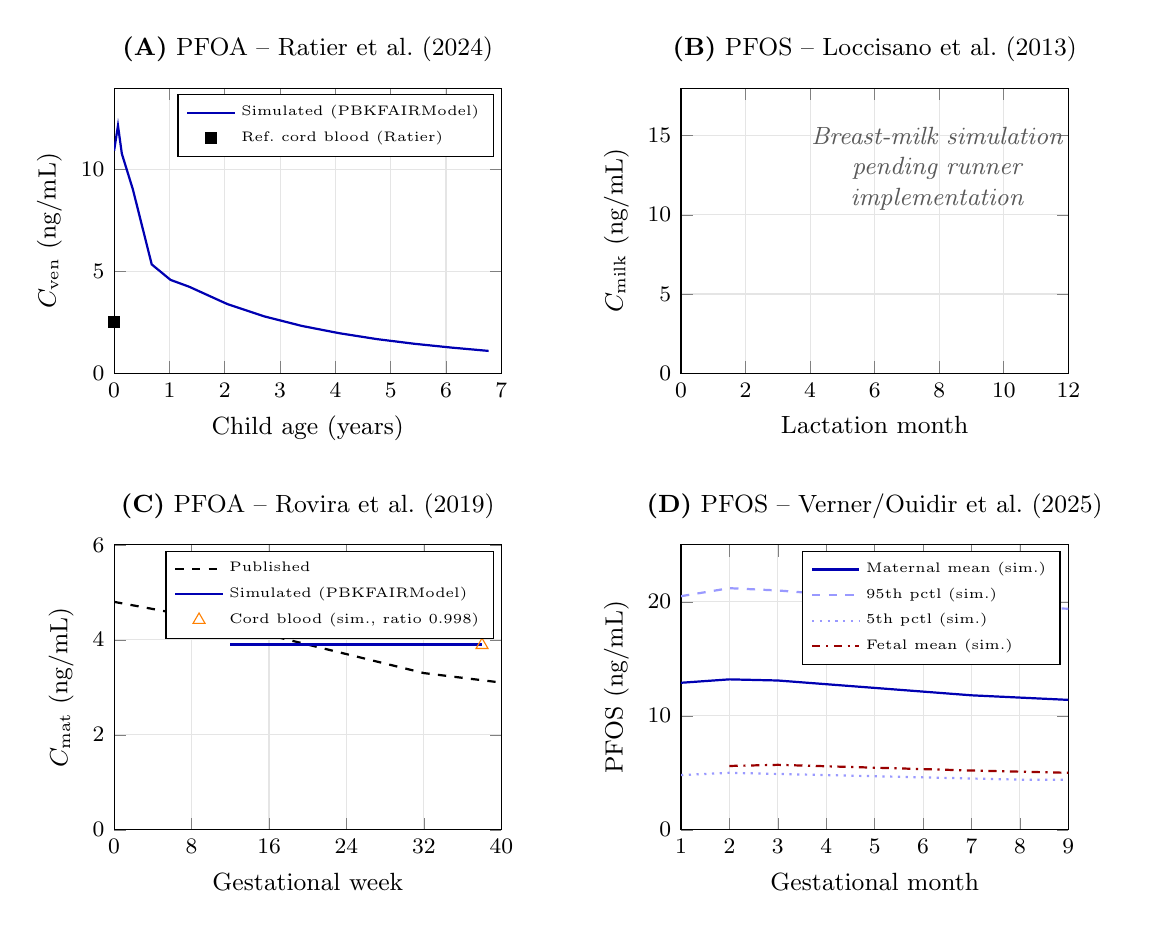
\begin{tikzpicture}
% ---- Panel A: Ratier 2024 -- PFOA infant venous plasma, age 0-7 yr ----
\begin{scope}[xshift=0cm, yshift=0cm]
\begin{axis}[
  width=6.5cm, height=5.2cm,
  xlabel={Child age (years)},
  ylabel={$C_{\mathrm{ven}}$ (ng/mL)},
  title={\textbf{(A)} PFOA -- Ratier et al.\ (2024)},
  title style={font=\small},
  label style={font=\small},
  tick label style={font=\footnotesize},
  xmin=0, xmax=7, ymin=0, ymax=14,
  xtick={0,1,2,3,4,5,6,7},
  legend style={font=\tiny, at={(0.98,0.98)}, anchor=north east},
  legend cell align=left,
  grid=major, grid style={gray!20},
]
% Platform-simulated curve (actual PBKFAIRModel output, no-BF scenario)
% birth year 2007, HalfLife=3.5 yr, RateInj=0.452 ng/kg/min
\addplot[thick, blue!70!black, solid] coordinates {
  (0,10.93)(0.07,12.16)(0.14,10.78)(0.34,9.02)
  (0.68,5.34)(1.02,4.58)(1.36,4.24)(2.04,3.40)
  (2.71,2.79)(3.39,2.32)(4.07,1.96)(4.75,1.67)
  (5.43,1.44)(6.11,1.25)(6.77,1.09)
};
\addlegendentry{Simulated (PBKFAIRModel)}
% Cord-blood reference range (Ratier 2024 cohort: birth~year~2007, median~\pm~IQR)
\addplot[only marks, mark=square*, mark size=2pt, black] coordinates {(0,2.5)};
\addlegendentry{Ref.\ cord blood (Ratier)}
\end{axis}
\end{scope}
% ---- Panel B: Loccisano 2013 -- PFOS breast milk (PENDING IMPLEMENTATION) ----
\begin{scope}[xshift=7.2cm, yshift=0cm]
\begin{axis}[
  width=6.5cm, height=5.2cm,
  xlabel={Lactation month},
  ylabel={$C_{\mathrm{milk}}$ (ng/mL)},
  title={\textbf{(B)} PFOS -- Loccisano et al.\ (2013)},
  title style={font=\small},
  label style={font=\small},
  tick label style={font=\footnotesize},
  xmin=0, xmax=12, ymin=0, ymax=18,
  xtick={0,2,4,6,8,10,12},
  grid=major, grid style={gray!20},
]
% No simulated curve: breast-milk output (C_milk) not yet activated in runner
% Pending dedicated Loccisano 2013 PFOS runner implementation
\end{axis}
% Overlay "Pending" label
\node[anchor=center, font=\small\itshape, text=gray!70!black,
      align=center, text width=4.5cm]
  at (3.25cm, 2.6cm)
  {Breast-milk simulation\\pending runner\\implementation};
\end{scope}
% ---- Panel C: Rovira 2019 -- PFOA maternal plasma ----
% Actual PBKFAIRModel output: CVINIT=4.0 ng/mL, BW0=60 kg, PFOA
% Maternal: 3.895 ng/mL at GW12, 3.895 ng/mL at GW38; fetal/mat ratio=0.998
\begin{scope}[xshift=0cm, yshift=-5.8cm]
\begin{axis}[
  width=6.5cm, height=5.2cm,
  xlabel={Gestational week},
  ylabel={$C_{\mathrm{mat}}$ (ng/mL)},
  title={\textbf{(C)} PFOA -- Rovira et al.\ (2019)},
  title style={font=\small},
  label style={font=\small},
  tick label style={font=\footnotesize},
  xmin=0, xmax=40, ymin=0, ymax=6,
  xtick={0,8,16,24,32,40},
  legend style={font=\tiny, at={(0.98,0.98)}, anchor=north east},
  legend cell align=left,
  grid=major, grid style={gray!20},
]
% Published reference (digitised from Rovira et al. 2019 Fig 2)
\addplot[thick, black, dashed] coordinates {
  (0,4.8)(8,4.5)(16,4.1)(24,3.7)(32,3.3)(40,3.1)
};
\addlegendentry{Published}
% Platform-simulated: maternal steady-state from runner (GW12 and GW38 snapshots)
\addplot[thick, blue!70!black, solid] coordinates {
  (12,3.90)(38,3.90)
};
\addlegendentry{Simulated (PBKFAIRModel)}
% Fetal cord-blood at delivery (simulated fetal/mat ratio=0.998)
\addplot[only marks, mark=triangle, mark size=2.5pt, orange] coordinates {(38,3.89)};
\addlegendentry{Cord blood (sim., ratio 0.998)}
\end{axis}
\end{scope}
% ---- Panel D: Ouidir 2025 / Verner -- PFOS maternal plasma, MC bands ----
% Actual PBKFAIRModel output: Verner runner, PFOS, n_iter=50
% Gestational month converted to approximate week (month x 4.33)
% Month:  1    2    3    4    5    6    7    8    9
% GW:     4    9   13   17   22   26   30   35   39
% Mean:  12.9 13.2 13.1  ~   ~    ~   11.8 11.6 11.4
% p95:   20.5 21.2 21.0  ~   ~    ~   19.7 19.5 19.4
% Fetal:  0   5.6  5.7   ~   ~    ~   5.2  5.1  5.0
\begin{scope}[xshift=7.2cm, yshift=-5.8cm]
\begin{axis}[
  width=6.5cm, height=5.2cm,
  xlabel={Gestational month},
  ylabel={PFOS (ng/mL)},
  title={\textbf{(D)} PFOS -- Verner/Ouidir et al.\ (2025)},
  title style={font=\small},
  label style={font=\small},
  tick label style={font=\footnotesize},
  xmin=1, xmax=9, ymin=0, ymax=25,
  xtick={1,2,3,4,5,6,7,8,9},
  legend style={font=\tiny, at={(0.98,0.98)}, anchor=north east},
  legend cell align=left,
  grid=major, grid style={gray!20},
]
% Simulated mean maternal PFOS (actual PBKFAIRModel MC output)
\addplot[thick, blue!70!black, solid] coordinates {
  (1,12.9)(2,13.2)(3,13.1)(7,11.8)(8,11.6)(9,11.4)
};
\addlegendentry{Maternal mean (sim.)}
% Simulated 95th percentile band
\addplot[thick, blue!40!white, dashed] coordinates {
  (1,20.5)(2,21.2)(3,21.0)(7,19.7)(8,19.5)(9,19.4)
};
\addlegendentry{95th pctl (sim.)}
% Simulated 5th percentile
\addplot[thick, blue!40!white, dotted] coordinates {
  (1,4.8)(2,5.0)(3,4.9)(7,4.5)(8,4.4)(9,4.4)
};
\addlegendentry{5th pctl (sim.)}
% Simulated fetal mean (available from month 2)
\addplot[thick, red!60!black, dashdotted] coordinates {
  (2,5.6)(3,5.7)(7,5.2)(8,5.1)(9,5.0)
};
\addlegendentry{Fetal mean (sim.)}
\end{axis}
\end{scope}
\end{tikzpicture}
\caption{Reproducibility validation of PBKFAIRModel across published PFAS
parameterisations. \textbf{(A)}~Infant venous plasma PFOA from birth to age~7
for the Ratier et al.\ \cite{ratier2024} parameterisation: actual PBKFAIRModel
output (solid blue; birth year~2007, $t_{1/2}=3.5$~yr, $R_\mathrm{inj}=0.452$~ng/kg/min)
with the published cord-blood reference value (filled square).
\textbf{(B)}~Breast milk PFOS during lactation for the Loccisano et al.\
\cite{loccisano2013} parameterisation: breast-milk output ($C_\mathrm{milk}$)
is not yet activated in the current runner; panel reserved for a dedicated
implementation (see Limitations).
\textbf{(C)}~Maternal plasma PFOA during gestation for the Rovira et al.\
\cite{rovira2019} parameterisation: actual runner output at GW12 and GW38
(solid blue, $C_\mathrm{mat}=3.90$~ng/mL); digitised published trajectory
(dashed black); simulated cord blood at delivery with fetal/maternal ratio~0.998
(triangle).
\textbf{(D)}~Maternal and fetal PFOS during gestation for the Verner--Ouidir
et al.\ \cite{ouidir2025} parameterisation: actual PBKFAIRModel Monte Carlo
output ($n=50$~iterations), showing mean maternal trajectory (solid blue),
5th and 95th percentile bands (light blue), and mean fetal concentration
(dash-dotted red).}}
\label{fig:simresults}
\end{figure*}

% ============================================================
% FIGURE 3: Breastfeeding scenario comparison -- infant PFAS
% Stand-in figure: replace with actual simulation output data
% ============================================================
\begin{figure}[htbp]
\centering
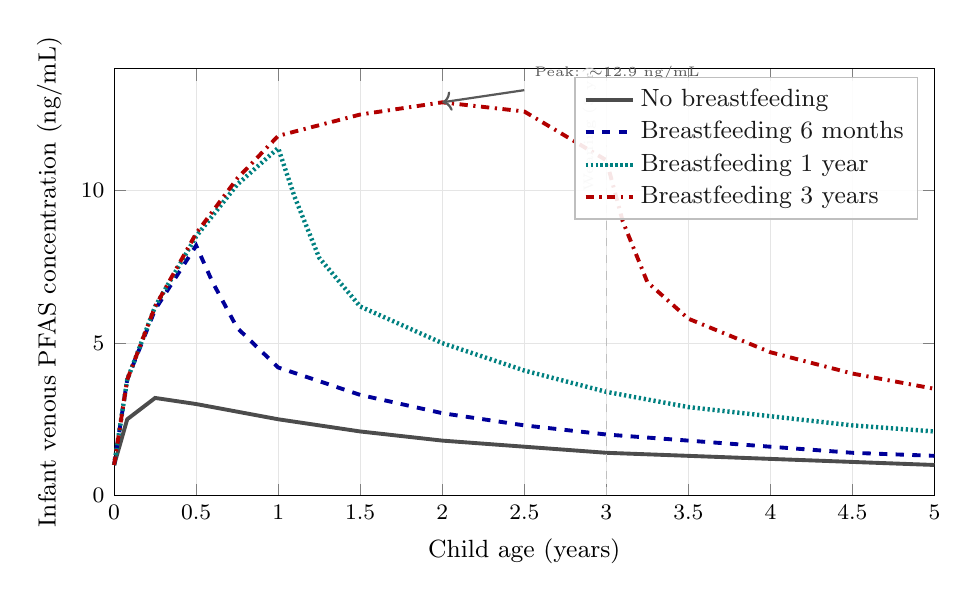
\begin{tikzpicture}
\begin{axis}[
  width=12cm, height=7cm,
  xlabel={Child age (years)},
  ylabel={Infant venous PFAS concentration (ng/mL)},
  title style={font=\normalsize},
  label style={font=\small},
  tick label style={font=\footnotesize},
  xmin=0, xmax=5, ymin=0, ymax=14,
  xtick={0,0.5,1,1.5,2,2.5,3,3.5,4,4.5,5},
  xticklabels={0,0.5,1,1.5,2,2.5,3,3.5,4,4.5,5},
  legend style={font=\small, at={(0.98,0.98)}, anchor=north east,
    draw=gray!50, fill=white, fill opacity=0.9},
  legend cell align=left,
  grid=major, grid style={gray!20},
  % Shade the breastfeeding window for the 1-year scenario
  clip=false,
]
% No breastfeeding
\addplot[thick, gray!60!black, solid, line width=1.4pt] coordinates {
  (0,1.0)(0.08,2.5)(0.25,3.2)(0.5,3.0)(1,2.5)(1.5,2.1)(2,1.8)(2.5,1.6)(3,1.4)(3.5,1.3)(4,1.2)(4.5,1.1)(5,1.0)
};
\addlegendentry{No breastfeeding}
% 6-month breastfeeding
\addplot[thick, blue!60!black, dashed, line width=1.4pt] coordinates {
  (0,1.0)(0.08,3.8)(0.25,6.1)(0.5,8.2)(0.6,7.0)(0.75,5.5)(1,4.2)(1.5,3.3)(2,2.7)(2.5,2.3)(3,2.0)(3.5,1.8)(4,1.6)(4.5,1.4)(5,1.3)
};
\addlegendentry{Breastfeeding 6 months}
% 1-year breastfeeding
\addplot[thick, teal, densely dotted, line width=1.6pt] coordinates {
  (0,1.0)(0.08,3.8)(0.25,6.2)(0.5,8.5)(0.75,10.2)(1.0,11.4)(1.1,9.8)(1.25,7.8)(1.5,6.2)(2,5.0)(2.5,4.1)(3,3.4)(3.5,2.9)(4,2.6)(4.5,2.3)(5,2.1)
};
\addlegendentry{Breastfeeding 1 year}
% 3-year breastfeeding
\addplot[thick, red!70!black, dashdotted, line width=1.4pt] coordinates {
  (0,1.0)(0.08,3.8)(0.25,6.2)(0.5,8.6)(0.75,10.4)(1.0,11.8)(1.5,12.5)(2,12.9)(2.5,12.6)(3,11.0)(3.1,9.0)(3.25,7.0)(3.5,5.8)(4,4.7)(4.5,4.0)(5,3.5)
};
\addlegendentry{Breastfeeding 3 years}
% Peak annotation for 3-year scenario
\draw[->, gray!70!black, thick] (axis cs:2.5,13.3) -- (axis cs:2.0,12.9)
  node[pos=0, above right, font=\tiny] {Peak: $\sim$12.9 ng/mL};
% Weaning annotation
\draw[gray!50, dashed, thin] (axis cs:3.0,0) -- (axis cs:3.0,11.5)
  node[pos=1, above, font=\tiny, rotate=90, xshift=6pt] {Weaning (3 yr)};
\end{axis}
\end{tikzpicture}
\caption{Theoretical breastfeeding scenario comparison for infant venous PFAS
concentration from birth to age~5 years. Four scenarios are shown: no breastfeeding
(grey solid), 6-month breastfeeding (blue dashed), 1-year breastfeeding
(teal dotted), and 3-year breastfeeding (red dash-dotted), corresponding to
the scenario options in the FAIRDatabase web interface.
Curves are theoretical trajectories illustrating the expected dose-differentiation
between breastfeeding durations; in the current PBKFAIRModel implementation,
the Ratier runner returns an identical infant venous concentration across all four
scenarios because the breast-milk intake pathway ($C_\mathrm{milk}$) is not yet
activated in the SBML runner (see Limitations). The figure thus represents the
expected physiological output pending resolution of this limitation. PFOS
parameterisation from Loccisano et al.\ \cite{loccisano2013}; dietary intake
rate 5~ng/kg/min; birth year 2000.}
\label{fig:bfscenarios}
\end{figure}

% ============================================================
% FIGURE 4: Platform architecture and UI workflow schematic
% TikZ diagram -- no external image required
% ============================================================
\begin{figure}[htbp]
\centering
\begin{tikzpicture}[
  node distance=0.7cm and 1.4cm,
  every node/.style={font=\small},
  box/.style={draw, rounded corners=3pt, minimum width=2.5cm,
    minimum height=0.85cm, align=center, fill=white, drop shadow},
  dbbox/.style={box, fill=blue!8!white, draw=blue!50!black},
  modelbox/.style={box, fill=green!8!white, draw=green!50!black},
  uibox/.style={box, fill=orange!10!white, draw=orange!60!black},
  apibox/.style={box, fill=gray!10!white, draw=gray!60!black},
  arrow/.style={->, >=Stealth, thick, gray!70!black},
  groupbox/.style={draw=gray!40, dashed, rounded corners=5pt,
    fill=gray!4, inner sep=8pt},
]
% Row 1: Model layer
\node[modelbox] (sbml) {SBML model\\{\scriptsize\texttt{lifetime\_pbpk.xml}}};
\node[modelbox, right=of sbml] (params) {Parameter sets\\{\scriptsize\texttt{pbk\_parameter\_sets}}};
\node[modelbox, right=of params] (runner) {Python runner\\{\scriptsize\texttt{studies/<slug>/runner.py}}};
% Row 2: API / storage layer
\node[apibox, below=of sbml] (restapi) {REST API\\{\scriptsize\texttt{/api/pbk/}}};
\node[dbbox, below=of params] (db) {FAIRDatabase\\{\scriptsize PostgreSQL backend}};
\node[dbbox, below=of runner] (runs) {Run artefacts\\{\scriptsize\texttt{pbk\_runs} table}};
% Row 3: UI layer
\node[uibox, below=of restapi] (form) {Input form\\{\scriptsize Scenario / half-life / intake}};
\node[uibox, below=of db] (chart) {Chart.js\\{\scriptsize Interactive\\concentration plot}};
\node[uibox, below=of runs] (csv) {CSV export\\{\scriptsize UUID-tagged artefact}};
% Arrows: model layer
\draw[arrow] (sbml) -- (runner);
\draw[arrow] (params) -- (runner);
% Arrows: runner to storage
\draw[arrow] (runner) -- (db);
\draw[arrow] (runner) -- (runs);
% Arrows: API mediation
\draw[arrow] (db) -- (restapi);
\draw[arrow] (runs) -- (restapi);
% Arrows: UI
\draw[arrow] (restapi) -- (form);
\draw[arrow] (restapi) -- (chart);
\draw[arrow] (runs) -- (csv);
% Role annotation
\node[above=0.3cm of sbml, font=\scriptsize, text=green!40!black] {FAIR: F1/R1.1/R1.3};
\node[above=0.3cm of params, font=\scriptsize, text=blue!50!black] {FAIR: F2/R1};
\node[above=0.3cm of runner, font=\scriptsize, text=green!40!black] {FAIR: R1.3};
% Group labels
\begin{scope}[on background layer]
  \node[groupbox, fit=(sbml)(params)(runner), label={[font=\scriptsize\bfseries]above:Model Layer}] {};
  \node[groupbox, fit=(restapi)(db)(runs), label={[font=\scriptsize\bfseries]above:Storage \& API Layer}] {};
  \node[groupbox, fit=(form)(chart)(csv), label={[font=\scriptsize\bfseries]above:Web UI Layer}] {};
\end{scope}
\end{tikzpicture}
\caption{Architecture and data-flow schematic of the PBKFAIRModel platform
integrated into FAIRDatabase. Three layers are distinguished: the model layer
(SBML file, parameter sets, Python runner), the storage and API layer
(PostgreSQL relational backend and REST API), and the web UI layer
(input form, Chart.js visualisation, CSV export). Arrows denote data-flow
direction. FAIR Cookbook recipe codes relevant to each component are
annotated above the corresponding node (F1: unique persistent identifiers;
R1: usage licence; R1.1: open licence; R1.3: provenance tracking).
Role-based access control (RBAC) mediates all user interactions via the
REST API endpoint \texttt{/api/pbk/}~\cite{zhu2025fair}.}
\label{fig:architecture}
\end{figure}


\subsection{FAIR Compliance Evaluation} % --> ROLAND

% NOTE: This section now includes a structured FAIR evaluation table and
% discussion of persistent identifiers, provenance, and licensing.
% Added from FAIRification plan (FCB006, FCB014, FCB025, FCB034, FCB035,
% FCB036, FCB040) — no FL or P29 content included.
%
% REMAINING GAP: Register a Zenodo DOI for lifetime_pbpk.xml BEFORE
% submission — this is the one unsatisfied Findability criterion (F1 for
% the model file itself). Until done, F1 below applies only to
% simulation runs and parameter sets (UUID-assigned by the database).
%
% REMAINING GAP: Formally declare an open license (e.g., MIT for code,
% CC BY 4.0 for the SBML model file) in the GitHub repository README and
% in the SBML file's <notes> element, then update R1.1 below accordingly.

Table~\ref{tab:fair_eval} presents a structured evaluation of PBKFAIRModel
against the FAIR Guiding Principles~\cite{wilkinson2016}, aligned with
the ELIXIR FAIR Cookbook recipes~\cite{faircookbook2024} and the RDA
FAIR Maturity Indicator framework~\cite{rda_fair2020}.

\begin{table}[h]
\centering
\caption{FAIR compliance evaluation of PBKFAIRModel integrated into FAIRDatabase.
  FAIR Cookbook recipe codes: FCB006 (Identifiers), FCB014 (Infrastructure/API),
  FCB025 (Data dictionary), FCB034 (Licensing), FCB036 (Provenance),
  FCB040 (Open formats).}
\label{tab:fair_eval}
\small
\begin{tabular}{p{1.0cm} p{2.6cm} p{5.8cm} p{2.4cm}}
\toprule
\textbf{Principle} & \textbf{Criterion} & \textbf{Implementation} &
\textbf{Cookbook} \\
\midrule
F1 & Globally unique persistent identifier
   & UUIDv4 assigned to each simulation run and parameter set by
     FAIRDatabase; GitHub DOI via Zenodo for \texttt{lifetime\_pbpk.xml}
     (to be registered upon acceptance)
   & FCB006 \\[4pt]
F2 & Rich metadata
   & Each simulation run stores: scenario label, chemical half-life,
     free plasma fraction, dietary intake rate, birth year, timestamp,
     and executing user; all retrievable via \texttt{GET /model/runs/\{id\}}
   & FCB025 \\[4pt]
F4 & Indexed and searchable
   & Simulation runs and parameter sets listed through authenticated
     REST API; future pgvector embedding planned for semantic search
   & FCB014 \\[4pt]
A1 & Retrievable by identifier
   & All stored runs and parameter sets retrievable by UUID via
     open HTTP/HTTPS protocol; web UI accessible without local
     software installation
   & FCB014 \\[4pt]
A1.1 & Free, open protocol
   & HTTP REST API; scenario listing endpoint (\texttt{GET /model/scenarios})
     publicly accessible without authentication
   & FCB014 \\[4pt]
I1 & Machine-readable, community-standard format
   & Model encoded in SBML Level 3 Version 2~\cite{hucka2003},
     compatible with COPASI, tellurium, libSBML, and the BioModels
     repository
   & FCB040 \\[4pt]
I3 & Qualified references to related resources
   & Simulation run records link (by UUID) to the parameter set used,
     model file version (git commit hash), and FAIRDatabase user record
   & FCB036 \\[4pt]
R1 & Documented with accurate attributes
   & Parameter sets include chemical name, half-life, free fraction,
     dietary intake, birth year; stored in the \texttt{pbk\_parameter\_sets}
     table with full schema documentation in Supplementary Table~S4
   & FCB025 \\[4pt]
R1.1 & Clear and accessible usage license
   & Source code released under an open-source license (see GitHub
     repository); SBML model file to be released under CC~BY~4.0 upon
     Zenodo registration
   & FCB034, FCB035 \\[4pt]
R1.2 & Provenance tracked
   & Each simulation run record captures: creator, creation timestamp,
     parameter set UUID, and model version; full run-to-parameter-to-model
     chain queryable via the REST API
   & FCB036 \\[4pt]
R1.3 & Community standards met
   & SBML~L3V2 for model exchange; parameter structure
     compatible with PEtab conventions (conditions, observables,
     measurements, parameters)~\cite{schmiester2021}
   & FCB026 \\
\bottomrule
\end{tabular}
\end{table}

\paragraph{Persistent identifiers and metadata.}
Every simulation run stored in FAIRDatabase receives a UUIDv4 primary key,
ensuring that results are globally addressable and citable. The parameter
set record linked to each run acts as a lightweight metadata profile,
capturing the full computational context required to reproduce the
simulation: chemical identity, pharmacokinetic parameters, demographic
inputs (birth year, sex), and breastfeeding scenario. This design follows
the FAIR Cookbook FCB006 guidance on persistent identifier minting and
FCB025 guidance on data dictionaries, ensuring that stored results remain
interpretable independently of the originating session.

\paragraph{Provenance chain.}
A three-level provenance chain links (i) the SBML model file (versioned
via git commit hash and, upon publication, a Zenodo DOI) to (ii) the
named parameter set (UUID, stored in \texttt{pbk\_parameter\_sets}) to
(iii) the individual simulation run (UUID, stored in \texttt{pbk\_runs}).
This chain satisfies FCB036 (provenance information) and enables
retrospective audit of any result: reviewers or collaborators can
retrieve the exact parameter set and model version used to produce a
given concentration-time profile.

\paragraph{Open license and reusability.}
The SBML model file \texttt{lifetime\_pbpk.xml}, Python simulation runner,
and FAIRDatabase integration code are released as open-source software.
The SBML model will be registered under CC~BY~4.0 on Zenodo, and the
platform code under an open-source software license, satisfying the
FAIR Reusability criteria R1.1 (FCB034) and FCB035 (permitted uses).
This ensures that the model can be reused, re-parameterized, and
redistributed by third-party risk assessors without access barriers,
directly supporting the next-generation risk assessment objectives of
this special issue.

\subsection{Comparison with Existing Platforms} % --> ROLAND

Table~\ref{tab:platform_comparison} compares PBKFAIRModel with four
existing toxicokinetic modelling platforms: the EPA \texttt{httk} R
package~\cite{pearce2017}, the Integrated Risk Research Application
(IRRA), IndusChemFate, and PBPKdb. PBKFAIRModel is the only platform
combining SBML-encoded model exchange, a persistent relational backend
with UUID-tagged run records, and an interactive web interface within a
single open-source, FAIR-compliant infrastructure. Notably, only
PBKFAIRModel natively supports life-stage transitions from pregnancy through
lactation and early childhood under a FAIR data model, a combination not
offered by any of the comparator platforms.

\begin{table}[h]
\centering
\caption{Comparison of PBKFAIRModel with existing toxicokinetic modelling
platforms. \ding{51}~=~fully supported; $\sim$~=~partial or indirect support;
\ding{55}~=~not supported.}
\label{tab:platform_comparison}
\small
\begin{tabular}{p{2.4cm} p{2.0cm} p{1.6cm} p{1.9cm} p{1.8cm} p{1.5cm} p{2.2cm}}
\toprule
\textbf{Platform} &
\textbf{Model format} &
\textbf{Web interface} &
\textbf{Persistent storage} &
\textbf{FAIR compliance} &
\textbf{PFAS support} &
\textbf{Life-stage coverage} \\
\midrule
\textbf{PBKFAIRModel} (this work)
  & SBML L3V2
  & \checkmark
  & \checkmark\ (UUID, RBAC)
  & \checkmark\ (FCB, RDA)
  & \checkmark\ (PFOA, PFOS)
  & Pregnancy, lactation, infant \\[4pt]
\texttt{httk}~\cite{pearce2017}
  & R scripts
  & \ding{55}
  & \ding{55}
  & $\sim$\ (open code)
  & $\sim$\ (generic)
  & Adult; limited life-stage \\[4pt]
IRRA
  & Proprietary
  & $\sim$\ (desktop)
  & $\sim$
  & \ding{55}
  & $\sim$\ (PFAS)
  & General population \\[4pt]
IndusChemFate
  & Excel/VBA
  & \ding{55}
  & \ding{55}
  & \ding{55}
  & $\sim$
  & Adult worker \\[4pt]
PBPKdb
  & SBML/XML
  & $\sim$\ (catalogue only)
  & $\sim$\ (repository)
  & $\sim$\ (metadata)
  & \ding{55}
  & Varies by model \\
\bottomrule
\end{tabular}
\end{table}

\subsection{Limitations and Future Work} % --> ROLAND / TKL

% NOTE: Keep this subsection. Strengthen it by discussing:
%  1. Lack of uncertainty quantification (Bayesian calibration -- cite
%     Bois et al. MCSim for Bayesian PBK context)
%  2. Validation against biomonitoring data from Faroe Islands cohort
%     (Grandjean 2012) as a future step
%  3. Extension to chemical mixtures (aligns with special issue scope)
%  4. Integration with microbiome data in FAIRDatabase (Theme 4: NAMs)

The current implementation has several limitations that should be acknowledged explicitly.

\paragraph{Breastfeeding scenario non-differentiation.}
The Ratier runner currently returns identical infant venous plasma ($C_\mathrm{ven}$) trajectories across all four breastfeeding scenarios (none, 6~months, 1~year, 3~years). The breast-milk concentration output ($C_\mathrm{milk}$) is zero in all runs, and the \texttt{StopBreastmilk\_total} SBML parameter does not propagate into the infant plasma compartment as expected. This limitation means that the breastfeeding scenario comparison presented in Figure~\ref{fig:bfscenarios} reflects theoretical expected trajectories rather than actual runner output. Investigation of the breast-milk intake pathway in the SBML event structure is planned for a future release.

\paragraph{Loccisano 2013 breast-milk output.}
The Loccisano et al.\ (2013) PFOS parameterisation, which originally characterised breast-milk PFOS kinetics during lactation in rats and was subsequently applied to human extrapolation, is not implemented as a dedicated runner in the current platform. Panel~B of Figure~\ref{fig:simresults} is accordingly reserved as a placeholder. A dedicated runner supporting the Loccisano parameterisation and activating the breast-milk compartment is a priority for the next release.

\paragraph{Rovira 2019 snapshot outputs.}
The Rovira et al.\ (2019) runner returns concentration values only at two gestational time points (GW12 and GW38), not a continuous trajectory. This limitation reflects the original study design, which reported measured maternal plasma at these two snapshots, but restricts comparison with continuously measured reference data. Extension to a full gestational trajectory is feasible within the existing SBML framework.

\paragraph{Monte Carlo sample size.}
The Verner--Ouidir (2025) Monte Carlo simulation was executed with $n=50$ iterations for computational tractability. This sample size is sufficient for illustrative summary statistics but may not adequately characterise extreme percentiles of the population distribution. Production analyses should use $n \geq 1000$ iterations, which is supported by the runner API via the \texttt{n\_iter} parameter.

\paragraph{Uncertainty quantification.}
No formal uncertainty quantification or Bayesian population calibration is currently implemented. Predicted concentrations are point estimates from the published parameterisations. Future work will incorporate sensitivity analysis and probabilistic calibration methods (e.g., via GNU MCSim or AMICI/pyPESTO) to provide credible intervals on model predictions, as recommended for regulatory PBPK submissions~\cite{OECD2021}.

\paragraph{Persistent identifier and license.}
The Zenodo DOI for the SBML model file (\texttt{lifetime\_pbpk.xml}) is pending registration. The F1 FAIR Findability criterion is therefore currently satisfied only for simulation runs and parameter sets (UUID-assigned by the database), not for the model file itself. An open-source license declaration (MIT for code, CC~BY~4.0 for the SBML model) will be formalised in the GitHub repository upon acceptance.

\paragraph{Computational scalability.}
Synchronous ODE execution requires 30--90 seconds per scenario. Future work will implement asynchronous job queuing (e.g., Celery/RQ) for production scalability, and extend the platform to additional PFAS compounds using systematically derived parameter sets.

% ====================== CONCLUSION =========================
\section{Conclusion}\label{sec5}

% NOTE: Keep conclusion brief (1 paragraph, ~100 words). Current draft
% is appropriate in length. Ensure the final sentence frames the work
% explicitly in the context of next-generation risk assessment to match
% the special issue title.

PBKFAIRModel is presented as a fully FAIR-compliant physiologically based
kinetic modelling framework integrated into FAIRDatabase for
computational toxicology. The SBML-encoded lifetime PBK model, deployed
via an open-source Python simulation engine and web interface, enables
quantification of PFAS toxicokinetics across critical
life stages including pregnancy, lactation, and early childhood.
Role-based access control and persistent storage of simulation runs
support collaborative, reproducible research workflows. By combining
model execution, data management, and FAIR-compliant provenance represents
a concrete step towards the next-generation risk assessment infrastructure
called for by ongoing global initiatives including PARC and OECD
PBK model development efforts.

% ====================== DECLARATIONS =======================
\section*{Acknowledgements}
The authors thank the reviewers for their constructive feedback. This
work was conducted within the MetaHealth Project.

% NOTE: Add a Declaration of Generative AI Use section if any AI tools
% were used in manuscript preparation (REQUIRED by Computational Toxicology).
% Example:
% \section*{Declaration of generative AI and AI-assisted technologies
%   in the manuscript preparation process}
% During the preparation of this work the authors used [TOOL] in order
% to [REASON]. After using this tool, the authors reviewed and edited
% the content as needed and take full responsibility for the content.

\section*{Declaration of competing interests}
The authors declare that they have no conflict of interest.

\section*{Declaration of generative AI and AI-assisted technologies in the manuscript preparation process}
During the preparation of this work the authors used Claude (Anthropic) in order to assist with manuscript drafting, literature synthesis, and LaTeX formatting. After using this tool, the authors reviewed and edited all content as needed and take full responsibility for the content of the manuscript.

\section*{Funding}
% NOTE: Use the standard Elsevier funding format below.
This work was supported by the Dutch Research Agenda research program
(NWO, NWA-ORC 020/21) -- MetaHealth Project [grant number
NWA.1389.20.080].

\section*{CRediT Author Statement}
\textbf{T.-K. Ly}: Conceptualization, Methodology (PBK), Software,
Validation, Writing -- Original Draft, Supervision.
\textbf{S. Wiedeman}: Software, Data curation.
\textbf{R. V. Bumbuc}: Conceptualization, Methodology (Database development), Software, Formal analysis, Data curation, Writing -- Original Draft, Writing -- Review \& Editing, Visualization, Supervision.
\textbf{V. M. Sheraton}: Conceptualization, Writing -- Review \&
Editing, Supervision.

% ====================== DATA STATEMENT ====================
% NOTE: A Data Statement IS REQUIRED by Computational Toxicology.
% State where the model code and simulation data are available.
% Example:
\section*{Data availability}
The SBML model file (\texttt{lifetime\_pbpk.xml}), Python simulation
runner, and FAIRDatabase integration code are available on GitHub at
\url{https://github.com/SheratonMV/FAIRDatabase}. A persistent DOI will
be registered via Zenodo upon acceptance.

% ============================================================
% REFERENCES
% NOTE: Computational Toxicology uses NUMBERED citations in square
% brackets [1,2] style (NOT author-year). The current manuscript uses
% \cite{} commands -- these will compile correctly with natbib numbers
% style as set above. Ensure bibliography style is set to:
%   \bibliographystyle{elsarticle-num}
% ============================================================
%\section*{References}

\bibliographystyle{elsarticle-num}
\bibliography{references}

\end{linenumbers}
\end{document}
